% AUTHOR: ASHWIN ABRAHAM

\documentclass{beamer}
\usepackage{xcolor}
\usepackage{algpseudocode}
\usepackage{framed}
\usepackage{listings}
\usepackage{amsmath}
\usepackage{hyperref}
\hypersetup
{
colorlinks=true,
linkcolor=blue,
filecolor=magenta,      
urlcolor=cyan,
pdftitle={Parameterized verification through view abstraction},
pdfpagemode=FullScreen,
}
\usepackage[utf8]{inputenc}

\usetheme{Madrid}
\usecolortheme{default}


\title[] 
{Summary:\\Parameterized verification through view abstraction}


\author[Ashwin Abraham] 
{Ashwin Abraham}

\institute[IIT-B] 
{
    IIT Bombay
}

\date[2023]
{February 2023}

% \logo{\includegraphics[height=2cm]{iitb-logo.png}}


\begin{document}
    \frame{\titlepage}

    \begin{frame}
        \frametitle{Table of Contents}
        \tableofcontents    
    \end{frame}

    \section{Abstract}
    {
        \begin{frame}
            \frametitle{Abstract}
            \begin{itemize}
                \item This paper presents an efficient framework for automatic verification of systems with a parametric number of concurrent, communicating processes. 
                \item For each value of the parameter, the system has a finite number of processes.
                
                \item The problem of automatic verification is to ensure that the system behaves \textit{correctly} for every value of the parameter.
                \item We say that a system behaves \textit{correctly}, if it cannot reach a predefined set of \textit{bad} configuration from a predefined set of \textit{initial} configurations. 
                
                \item For simplicity, we model each process as a Finite State Machine, and assume all the processes are copies of each other.
                \item Here, we parametrize over the size of the system (the number of processes).
            \end{itemize}
        \end{frame}

        \begin{frame}
            \frametitle{An overview of our strategy for automatic verification}
            \begin{itemize}
                \item We extract a model for each process in the system.
                \item We extract an \textit{overapproximation} of the model to give an abstract model
                \item We determine the initial states and bad states in this abstract model
                \item Finally, we check if the bad states can be obtained from the initial states in this abstract model
            \end{itemize}
        \end{frame}
    }

    \section{Interprocess communication}
    {
        \begin{frame}
            \frametitle{The Topology of a system}
            \begin{itemize}
                \item The topology of a system refers to which processes can communicate with (ie inspect the state of) other processes.
                
                \item Some common topologies are:
                \begin{enumerate}
                    \item Linear Topology:\\Here the processes are ordered in an array and each process can distinguish the states to its left and those to its right. It can inspect the state of any of these processes.
                    \item Ring Topology:\\The processes are ordered in a ring, and each process can only inspect the state of the process next to it.
                    \item Tree Topology:\\The processes are arranged in a tree and each process can distinguish its parent process and child processes and inspect their states.
                    \item Multiset Topology:\\Each process can distinguish every other process and inspect their states.
                \end{enumerate}
            \end{itemize}
        \end{frame}

        \begin{frame}
            \frametitle{The Topology of a system}
            We can represent the topology of a system by a directed graph $G(V, E)$ where the vertices correspond to processes, and there is an edge from 
            vertex $A$ to vertex $B$ if process $A$ can inspect the state of process $B$.
            \begin{figure}
                \begin{center}
                    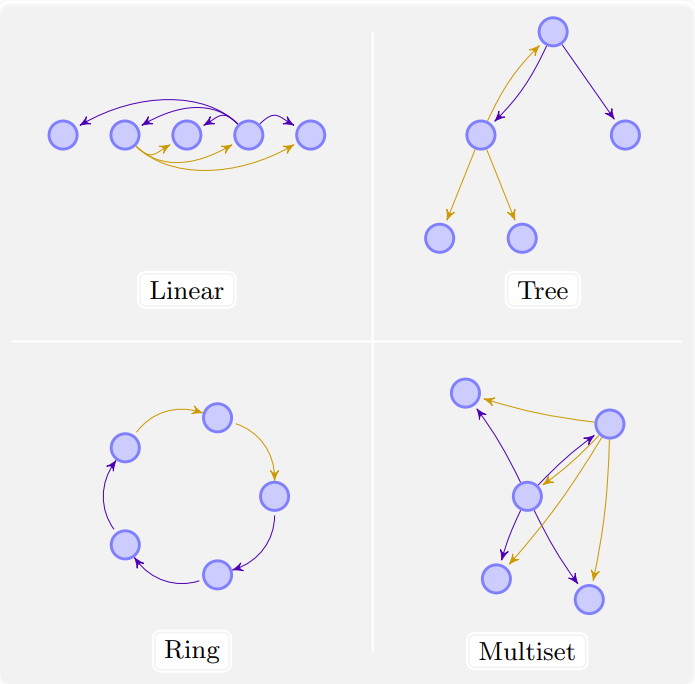
\includegraphics[scale=0.4]{images/topologies.png}
                    \caption{The graphs of the above mentioned topologies}
                \end{center}
            \end{figure}
        \end{frame}

        \begin{frame}
            \frametitle{Local and Global Transitions}
            \begin{itemize}
                \item If a process transitions from one state to another without needing to inspect the states of other processes, the transition is known as a local transition.
                \item On the other hand, if the transition is dependent on the states of other processes, the transition is called a global transition.
                \item A major issue that arises is that global transitions are not checked atomically. The state of an inspected process may change while other processes are still being inspected.
                \item The method presented provides an elegant solution to this issue.
            \end{itemize}
        \end{frame}

        \begin{frame}
            \frametitle{Other Transitions}
            \begin{itemize}
                \item Broadcast Transitions: Here, an arbitrary number of processes change their state simultaneously. 
                A broadcast transition has an initiator that causes a (possibly empty) subset of the processes that can inspect its state to transition.
                \item Rendezvous Transitions: Here a fixed number of processes change their state simultaneously. 
                \item Shared Variable Update: Here, the shared variable is a part of the state of multiple processes, and when it is updated by any of the 
                processes, the other processes change their state to reflect the updated value of the variable.
                \item Process Creation and Deletion make the topology of our system dynamic, but these can be reframed in terms of rendezvous transitions, as we 
                will see later.
            \end{itemize}
        \end{frame}
    }

    \section{Formalism}
    {
        \begin{frame}
            \frametitle{Formalism}
            To simplify our results, for now we will work with parametrized systems having identical processes and a linear topology, and that all transitions are either local or global. We assume for now that global checks are atomic, although we will soon drop this condition. We also assume that each process is governed by a finite state automaton.
            \begin{itemize}
                \item For a given topology, a parametrized system can be defined as the pair $\mathcal{P} = (\mathcal{Q}, \Delta)$, where $\mathcal{Q}$ is the set of \textit{local states} of each process and $\Delta$ is a set of transition rules over processes.
                \item A local transition rule will be of the form $s_{i} \rightarrow s'_{i}$, where $s_{i}, s'_{i} \in \mathcal{Q}$ refer to the states of the $i^{th}$ process before and after transition.
                \item A global rule is of the form $Q  j \sim i : s_{j} \in S \implies s_{i} \rightarrow s'_{i}$. Here $Q$ is a quantifier (either $\forall$ or $\exists$) and $\sim$ is some relation dependent on the topology of the system (for a linear topology it can be either $<$, $>$ or $\neq$)
                and $S$ is some subset of $\mathcal{Q}$.
            \end{itemize}
        \end{frame}

        \begin{frame}
            \frametitle{Formalism}
            \begin{itemize}
                \item The configuration $c$ of the system is a word over the alphabet $\mathcal{Q}$, ie, an array of states. We denote the set of all configurations as $\mathcal{C}$.
                \item $\left|c\right|$ denotes the number of processes. This is the parameter with which we parametrize the system.
                \item $c_{i}$ denotes the state of the $i^{th}$ process in configuration $c$, for $1 \leq i \leq \left|c\right|$.
                \item For a local rule $\delta \in \Delta$ such that $\delta = a \rightarrow b$, we say $c' = \delta(c, i)$ if $c'$ is the result of applying $\delta$ on the $i^{th}$ process.
                In particular, for $\delta(c, i)$ to be defined, $c_{i}$ must be $a$, and $\delta(c, i)_{i}$ will be $b$.
                \item For a global rule $\delta \in \Delta$ such that $\delta = Q j \sim i: s_{j} \in S \implies a \rightarrow b$, $\delta(c, i)$ is defined iff $c_{i} = a$, and the condition $Q j \sim i: s_{j} \in S$ is satisfied. In this case, $\delta(c, i)_{i} = b$.
                \item We write $c \xrightarrow[]{\delta} c'$ if $c' = \delta(c, i)$ for some $i \in \{1 \dots c\}$, and we define $\xrightarrow[]{*}$ as the reflexive and transitive closure of $\xrightarrow[]{\delta}$ (possibly with different $\delta$s).
            \end{itemize}
        \end{frame}

        \begin{frame}
            \frametitle{Reachability}
            \begin{itemize}
                \item We say that a configuration $c'$ is reachable from $c$ if $c \xrightarrow[]{*} c'$.
                \item The \textit{reachability problem} is defined by a parametrized system $\mathcal{P} = (\mathcal{Q}, \Delta)$, a set of initial states $\mathcal{I} \subseteq \mathcal{C}(\mathcal{P})$ and a set of bad states $\mathcal{B} \subseteq \mathcal{C}(\mathcal{P})$. 
                \item We define the set $\mathcal{R}$ of reachable states as $\{c \in C: \exists c' \in \mathcal{I}, c' \xrightarrow[]{*} c\}$. We say a $\mathcal{P}$ is \textit{safe} with respect to $\mathcal{I}$, $\mathcal{B}$ iff $\mathcal{R} \cap \mathcal{B} = \emptyset$.
                \item In order to define the \textit{bad} set $\mathcal{B}$ independently of the parameter, we define it as the closure of a set of minimal bad configurations, ie $\mathcal{B} = \{c \in \mathcal{C}: \exists b \in B_{min} b \sqsubseteq c\}$, where $\sqsubseteq$ denotes 
                a relation (known as the \textit{covering} relation) dependent on the topology of the system (for a linear topology it'll be the subword relation).
                \item $\mathcal{I}$ and $\mathcal{R}$ are also defined independently of the parameter this way.
                \item $\mathcal{S}_{k}$ denotes $\{c \in S: \left|c\right| = k\}$ for $S = \mathcal{I}$, $\mathcal{B}$, $\mathcal{R}, \mathcal{C}$. 
            \end{itemize}
        \end{frame}
    }
    \section{Szymanski's Protocol}
    {
        \begin{frame}
            \frametitle{Szymanski's Protocol}
            \begin{itemize}
                \item Szymanski's Protocol is a protocol that is used to ensure mutually exclusive access to a resource for a finite number of processes.
                \item It is based on the analogy of a waiting room with an entry door and an exit door that gives access to the resource.
                \item Each process has a flag with $5$ possible values:
                \begin{itemize}
                    \item \textbf{0}: The process declares that it doesn't want to access the resource right now (it is outside the waiting room)
                    \item \textbf{1}: The process declares that it wants to enter the critical section, and it is outside the waiting room.
                    \item \textbf{2}: The process is waiting for other processes to enter the waiting room.
                    \item \textbf{3}: The process has just entered the waiting room.
                    \item \textbf{4}: The process is about to start or in the critical section.
                \end{itemize}
                \item The flag of a process can be read by every other process but can be changed only by itself.
            \end{itemize}            
        \end{frame}

        \begin{frame}
            \frametitle{Szymanski's Protocol}
            \begin{itemize}
                \item In the beginning, all the processes that request entry at roughly the same time, enter the waiting room one by one. 
                \item The last of these closes the entry door and waits for the processes of lower IDs to leave the waiting room and finish accessing the resources.
                \item Once the lower ID processes are done, they change their flags to \textbf{0} or \textbf{1} to indicate this. The last process finishing resource access causes the entry door to be opened.
                \item For now, we assume that all these checks can be done atomically.
            \end{itemize}
        \end{frame}

        \begin{frame}[fragile]
            \frametitle{Szymanski's Protocol}
            The pseudocode for this protocol is as follows:
            \begin{figure}
                \begin{center}
                    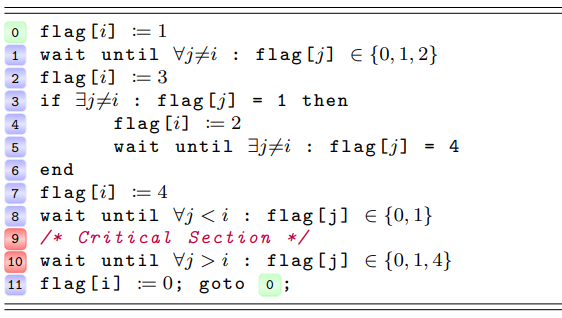
\includegraphics[scale=1]{images/codeimg.png}
                    % \caption{}
                \end{center}
            \end{figure}
        \end{frame}

        \begin{frame}
            \frametitle{Szymanski's Protocol}
            \begin{itemize}
                \item The configuration of the system here is a word over the alphabet $\{0, 1, \cdots 11\}$.
                \item The initial configuration of the system has all processes in state $0$.
                \item $\mathcal{I} = \{0, 0.0, 0.0.0 \cdots\}$
                \item The bad configurations are those where more than one process is in state $9$ or state $10$.
                \item $\mathcal{B} = \{9.9, 9.10, 10.9, 10.10, \cdots\}$
            \end{itemize}
        \end{frame}
    }
    \section{View Abstraction}
    {
        \begin{frame}
            \frametitle{Verification}
            \begin{itemize}
                \item The key insight here is that small instances of the system give enough information to predict the behaviour for all values of 
                the parameter.
                \item On a high level, we can say that this occurs because the patterns that occur for lower values of the parameter repeat themselves for larger values.
                \item The configurations for higher parameters cover those of lower parameters, in a sense.
                \item Our algorithm automatically detects a cutoff point $n$ such that we only need to compute $\mathcal{R}_{1}, \mathcal{R}_{2} \cdots \mathcal{R}_{n}$ to determine whether $\mathcal{R} \cap \mathcal{B} = \emptyset$. 
                \item To do this, we perform \textit{overapproximation}, where we abstract the system such that $R \subseteq R'$. Now if we are able to show $R' \cap B = \emptyset$, we can conclude that $R \cap B = \emptyset$.
            \end{itemize}
        \end{frame}

        \begin{frame}
            \frametitle{View Abstraction}
            \begin{itemize}
                \item We first focus only on \textit{atomically} checked global conditions. As mentioned earlier, we will remove this restriction soon.
                \item In \textit{view abstraction}, we consider the configurations from the perspective of a few \textit{fixed} number of processes. This abstraction is parametrized by $k$, the number of processes.
                \item The new construct made by considering the perspective of only the $k$ processes taken is called a \textit{view}.
                \item We have a certain freedom in choosing what information to discard and what to retain while constructing the view.
                \item For example, a simple example of a view would be a subword of the configuration $c$, with size $k$.
            \end{itemize}
        \end{frame}

        \begin{frame}
            \frametitle{The Subword View}
            \begin{itemize}
                \item Here, a view of a configuration $c$ with size $k$ is a subword of $c$ with size $k$.
                \item We denote the set of views by $\mathcal{V}$ and the set of views of size \textit{upto} $k$ by $\mathcal{V}_{k}$. Note that a view is also a valid configuration, and therefore $\mathcal{V}_{k} \subseteq \mathcal{C}$.
                \item We now define two functions:
                \begin{enumerate}
                    \item The \textit{abstraction} function $\alpha_{k}: \mathcal{C} \rightarrow 2^{\mathcal{V}_{k}}$ that maps a configuration to the set of all it's subwords of size at most $k$.
                    \begin{equation*}
                        \alpha_{k}(c) = \{v \in \mathcal{V}_{k}: v \sqsubseteq c\}, \forall c \in \mathcal{C}
                    \end{equation*}
                    \item We also define the \textit{abstraction} for subsets of $\mathcal{C}$ as $\alpha_{k}: 2^{\mathcal{C}} \rightarrow 2^{\mathcal{V}_{k}}$ as
                    \begin{equation*}
                        \alpha_{k}(S) = \{v \in \mathcal{V}_{k}: \exists c \in S: v \sqsubseteq c\} = \bigcup\limits_{c \in S} \alpha_{k}(c), \forall S \subseteq \mathcal{C}
                    \end{equation*}
                    \item The \textit{concretization} function $\gamma_{k}: 2^{\mathcal{V}_{k}} \rightarrow 2^\mathcal{C}$ that maps a set of views to the set of configurations that can be reconstructed from those views, ie
                    \begin{equation*}
                        \gamma_{k}(V) = \{c \in \mathcal{C}: \alpha_{k}(c) \subseteq V\}, \forall V \subseteq \mathcal{V}_{k}
                    \end{equation*}
                \end{enumerate}
            \end{itemize}
        \end{frame}

        \begin{frame}
            \frametitle{Galois Connection}
            \begin{itemize}
                \item We can order $2^{\mathcal{C}}$ and $2^{\mathcal{V}_{k}}$ by defining $x \leq y$ when $x \subseteq y$, $\forall x, y \in 2^{\mathcal{C}}$ or $\forall x, y \in 2^{\mathcal{V}_{k}}$.
                \item With this ordering, $\alpha_{k}$ and $\gamma_{k}$ become monotonic functions.
                \item $\forall V \subseteq \mathcal{V}_{k}, \alpha_{k}(\gamma_{k}(V)) \subseteq V$. This is because $\forall c \in \gamma_{k}(V)$, $\alpha_{k}(c) \subseteq V$ (by the definition of $\gamma_{k}$).
                \item $\forall S \subseteq C, S \subseteq \gamma_{k}(\alpha_{k}(S))$. This is because $c \in S \implies \alpha_{k}(c) \subseteq \alpha_{k}(S)$ (by monotonicity), which implies that $c \in \gamma_{k}(\alpha_{k}(S))$.
            \end{itemize}
            If $(A, \leq)$ and $(B, \leq)$ are two posets, we say two monotone functions $F: A \rightarrow B$ and $G: B \rightarrow A$ form a Galois Connection iff
            \begin{equation*}
                \forall a \in A, \forall b \in B, F(a) \leq b \Leftrightarrow a \leq G(b)
            \end{equation*}
            Now, $\alpha_{k}(A) \subseteq B \implies \gamma_{k}(\alpha_{k}(A)) \subseteq \gamma_{k}(B) \implies A \subseteq \gamma_{k}(B)$. Similiarly, we can prove the converse. Therefore, $\alpha_{k}$ and $\gamma_{k}$ form a Galois connection.
        \end{frame}

        \begin{frame}
            \frametitle{Monotonicity of $\gamma_{k}\alpha_{k}$}
            Lemma:
            \begin{equation*}
                \forall X \subseteq \mathcal{C}, X \subseteq \cdots \gamma_{2}(\alpha_{2}(X)) \subseteq \gamma_{1}(\alpha_{1}(X))
            \end{equation*}
            Proof:\\
            Since $\alpha_{k}(S) \subseteq \alpha_{k + 1}(S)$, we define $f_{k + 1}(S)$ as $\alpha_{k + 1}(S) - \alpha_{k}(S)$.
            Now, $\gamma_{k + 1}(\alpha_{k + 1}(X)) = \{c \in C: \alpha_{k + 1}(c) \subseteq \alpha_{k + 1}(X)\} = \{c \in C: \alpha_{k}(c) \cup f_{k + 1}(c) \subseteq \alpha_{k}(X) \cup f_{k + 1}(X)\}$.
            Since $\forall M, N, f_{k+1}(M) \cap \alpha_{k}(N) = \emptyset$, this is possible only when $\alpha_{k}(c) \subseteq \alpha_{k}(S)$ and $f_{k+1}(c) \subseteq f_{k + 1}(S)$, ie 
            \begin{equation*}
                \gamma_{k + 1}(\alpha_{k + 1}(S)) = \{c \in \mathcal{C}: \alpha_{k}(c) \subseteq \alpha_{k}(S) \land f_{k + 1}(c) \subseteq f_{k + 1}(S)\}
            \end{equation*}
            Therefore, 
            \begin{equation*}
                \gamma_{k + 1}(\alpha_{k + 1}(S)) \subseteq \{c \in \mathcal{C}: \alpha_{k}(c) \subseteq \alpha_{k}(S)\} = \gamma_{k}(\alpha_{k}(S))
            \end{equation*}
            This means that, although $\gamma_{k}(\alpha_{k}(S))$ is an overapproximation of $S$, as we increase the value of $k$, it becomes a better overapproximation. 
        \end{frame}

        \begin{frame}
            \frametitle{Some more terminology}
            If we find a $k$ such that $\mathcal{B} \cap \gamma_{k}(\alpha_{k}(\mathcal{R})) = \emptyset$, then we can conclude that $\mathcal{B} \cap \mathcal{R} = \emptyset$. This is the gist of our algorithm.\\
            Some more terminology:
            \begin{itemize}
                \item For a set of configurations $X \subseteq \mathcal{C}$, we define its \textit{post-image} $post(X)$ as the set $\{\delta(c, i) | c \in X, i \leq |c|, \delta \in \Delta\}$.
                \item We also define $post^{*}(X) = \{c \in \mathcal{C} : \exists c' \in X : c' \xrightarrow[]{*} c \}$. Since we deal only with transitions that do not change the topology of the system, $\mathcal{R}_{k} = post^{*}(\mathcal{I}_{k})$.
                \item We define the \textit{abstract post-image} of a set of views $V \subseteq \mathcal{V}_{k}$ as $\alpha_{k}(post(\gamma_{k}(V)))$. This represents the set of views that may be obtained after one transition of the system.
            \end{itemize}
        \end{frame}
    }

    \section{The Algorithm}
    {
        \begin{frame}
            \frametitle{The Algorithm}
            \begin{itemize}
                \item The algorithm determines a cutoff point $K$ such that a set of views $V \subseteq \mathcal{V}_{k}$ computed by the algorithm satisfy
                \begin{enumerate}
                    \item $Apost_{K}(V) \subseteq V$ and $\mathcal{R} \subseteq \gamma_{k}(V)$
                    \item $\gamma_{K}(V) \cap \mathcal{B} = \emptyset$
                \end{enumerate}
                \item If we can find such a $V$, then we can conclude that $\mathcal{R} \cap \mathcal{B} = \emptyset$.
                \item We iterate through the values of $k \in \mathbb{N}$ to find such a $V \subseteq \mathcal{V}_{k}$.
                \item For each value of $k$, we first check that $\mathcal{R}_{k} \cap \mathcal{B} = \emptyset$. If this is not the case, we can stop and say that the system is unsafe.
                \item We then proceed to calculate a fixed point of $Apost_{k}$ that contains $\alpha_{k}(\mathcal{I})$, ie $X \subseteq \mathcal{V}_{k}$ such that $\alpha_{k}(\mathcal{I}) \subseteq X$ and $Apost_{k}(X) \subseteq X$.
            \end{itemize}
        \end{frame}
    }

    % \section{Itemization and Linking}
    % {
    %     \begin{frame}
    %         \frametitle{Some Sorting Algorithms}
    %         There exist many sorting algorithms.
            

    %         Some algorithms run in $O(n^{2})$, such as:
            
    %         \begin{itemize}
    %             \item Bubble Sort
    %             \item Selection Sort
    %         \end{itemize}
            
    %         Some run in $O(n\log(n))$, such as:
            
    %         \begin{itemize}
    %             \item Merge Sort
    %             \item Quick Sort
    %         \end{itemize}
            
    %         Some run in $O(n)$ (for some arrays), such as:
            
    %         \begin{itemize}
    %             \item Counting Sort
    %         \end{itemize}
            
    %         And some are \textcolor{pink}{joke algorithms}, such as:
    %         \begin{itemize}
    %             \item <8-> \textit{\href{https://en.wikipedia.org/wiki/Bogosort}{Bogosort}}
    %             \item <9-> \textit{\href{https://quantumcomputing.stackexchange.com/questions/1265/what-can-we-learn-from-quantum-bogosort}{Quantum Bogosort}}
    %             \item <10-> \textit{\href{https://en.wikipedia.org/wiki/Slowsort}{Slowsort}}
    %         \end{itemize}
    %         which are \textbf{way worse} than even $O(n^{2})$!
    %     \end{frame}
    % }

    % \section{Matrices and Indented Equations}
    % {
    %     \begin{frame}
    %         \frametitle{Matrices and Indented Equations}
    %         We can also write matrices in \LaTeX{}!

    %         For example the (3x3) Identity Matrix can be written as:
    %         \begin{equation*}
    %             I_{3} = \begin{bmatrix}
    %                 1 & 0 & 0 \\
    %                 0 & 1 & 0 \\
    %                 0 & 0 & 1
    %             \end{bmatrix}
    %         \end{equation*}
            
    %         I can also indent equations, like so:
    %         \begin{align*}
    %             (\textbf{a}\cdot\textbf{b})^{2} &= (\sum a_{i}b_{i})^{2} \\
    %             &\leq (\sum a_{i})^{2}(\sum b_{i})^{2}
    %         \end{align*}
    %     \end{frame}
    % }
\end{document}